\documentclass[a4paper]{article}

\usepackage{color}
\usepackage{url}
\usepackage[utf8]{inputenc} % make weird characters work
\usepackage{graphicx}
\usepackage{makecell}

\usepackage[english,serbian]{babel}

\usepackage[unicode]{hyperref}
\hypersetup{colorlinks,citecolor=green,filecolor=green,linkcolor=blue,urlcolor=blue}
\renewcommand\theadalign{lc}
\renewcommand\theadfont{\bfseries}
\renewcommand\theadgape{\Gape[4pt]}
\renewcommand\cellalign{lc}
\renewcommand\cellgape{\Gape[4pt]}

\newtheorem{primer}{Primer}[section]

\begin{document}

\title{Generisanje test primera za programe u C-u korišćenjem Fuzz tehnike\\ \small{Seminarski rad u okviru kursa\\Metodologija stručnog i naučnog rada\\ Matematički fakultet}}

\author{Ana Đorđević, Mladen Lazić, Aleksandra Đurić\\ djordjevicana93@gmail.com, mladen.lazic93@hotmail.com, \\ aleksandradjuric@mail.ru}
\date{9.~april 2015.}
\maketitle

\abstract{
Najbitniji zahtevi prilikom implementacije softvera su njegova pouzdanost i performanse. Testiranjem se proverava stepen ispunjenosti ovih kriterijuma. U radu je izložen koncept Fuzz testiranja koje predstavlja glavno sredstvo za ispitivanje robusnosti razvijenog programa. Dat je i kratak pregled njegovih tipova, metoda koje koristi, prednosti i nedostataka. Implementirana je podrška za programe pisane u jeziku C. 
\tableofcontents
 
\newpage
 
\section{Uvod}
\label{sec:uvod}

Testiranje predstavlja važan deo životnog ciklusa razvoja softvera. Omogućava lakše uočavanje grešaka i propusta nastalih prilikom implementacije. Pored toga ono predstavlja i jedan od načina specifikacije problema. 
Kako i najmanji problem može uništiti uložen trud, u slučaju obimnih projekata nikada nije dovoljno testiranja.
S porastom složenosti projekta raste i značaj testiranja i provera softvera kako bi se izbegli ishodi koju mogu da unište ceo projekat.
Kako se greške ne mogu izbeći, potrebno ih je što je moguće ranije otkriti kako bi njihovo otklanjanje
bilo brže i jeftinije. Zbog prednosti koje se dobijaju najzastupljenije i trenutno najpopularnije metodologije razvoja promovišu paralelno pisanje testova i implementacije softvera. Ekstremno programiranje kao jedan od predstavnika agilnih metodologija posebno ističe razvoj vođen testovima i pisanje testova prihvatljivosti \cite{agilnirazvoj}.
Testiranje se sastoji od planiranja, gde se određuje predmet, cilj i razlog testiranja, zatim sledi dizajn testova koji određuje kako se sprovodi testiranje na osnovu test primera. Treća faza je implementacija testova iza koje sledi izvršavanje testova radi provere funkcionalnosti sistema. Kao poslednja faza se definiše evaluacija testova koja uključuje validnost izvršavanja testa, analizu izlaza i pregled dobijenih rezultata.


\section{Vrste testiranja}
\label{sec:vrste_testiranja}
Testiranje se može izvoditi na različite načine. Čest pristup je testiranje jedinice (eng~{\em Unit test}) gde se zasebno testira svaka programska 
komponenta, nezavisno od ostalih delova sistema. Takvo testiranje se može vršiti na podprogramima ili celinama sačinjenim od manjih komponenti.
U upotrebi je i integraciono testiranje kao proces verifikovanja spregnutosti među komponentama sistema. Uobičajene strategije integralnog testiranja se koriste kod hijerarhijski strukturiranog softvera. Savremene integrativne strategije više pažnje posvećuju arhitekturi sistema. Koristi se i sistemsko testiranje koje proverava ponašanje celog sistema uključujući aspekte kao što su bezbednost, brzina, preciznost ili performanse. Interfejsi ka drugim aplikacijama, pomoćnim programima, hardverskim uređajima ili okruženjima se takođe razmatraju na ovom nivou.
Veoma zastupljeni su i testovi prihvatljivosti koji proveravaju ponašanje sistema prema zahtevima naručioca softvera, koji formira tipične zadatke za koje se proverava ispunjenost zahteva. Pored toga, razlikujemo i instalaciono testiranje koje podrazumeva proveru softvera 
nakon instalacije u ciljnom okruženju. Ovaj način testiranja može se izvoditi prema zahtevima hardverske konfiguracije. Značajno je i regresiono testiranje koje testira sistem u ciklusima kako bi se proverilo da promene
nisu proizvele neželjene efekte. Regresioni testovi obezbeđuju da performanse novog sistema budu barem jednake performansama starog.
Konačno, primenjuje se i testiranje performansi koje uključuje proveru kapaciteta i vremena odziva. \\

U literaturi se sreću različite podele testiranja. Svaka je nastala kao posledica posmatranja različitih aspekata i pristupa provere programa. Jedna od opšte prihvaćenih podela je na testiranje crnom kutijom (eng~{\em Black Box Testing}), sivom kutijom (eng~{\em Grey Box Testing}) i belom kutijom (eng~{\em White Box Testing}) \cite{fuzzing}. U nastavku je dat opis navedenih vrsta. Tehnika sive kutije nije posebno razmatrana jer predstavlja kombinaciju druga dva pristupa. Kod ove strategije ne postoji pristup izvornom kodu, ali postoji pristup nekom segmentu softvera. Često je to pristup bazi podataka.

\subsection{Strategija crne kutije}
\label{subsec:crna_kutija}
Testiranje crnom kutijom je strategija koja zahteva da se program posmatra kao zatvoreni sistem kako bi se utvrdilo ponašanje programa na osnovu odgovarajućih ulaznih podataka. Ova strategija, za razliku od strategija bele kutije, ne zahteva poznavanje strukture i analizu
izvornog koda, već samo način funkcionisanja sistema koji se testira. Izvršava se tako sto se sistemu prosleđuju odgovarajući ulazni podaci a zatim se proverava da li je izlaz u skladu sa očekivanom specifikacijom funkcionalnosti sistema. Ova situacija je uobičajena prilikom testiranja web aplikacija ili web servisa gde se razmatra web strana koju je generisao server na osnovu unetih podataka. Strategija testiranja crne kutije obično nije najbolji pristup, ali je uvek opcija. Kao prednost ove strategije može se navesti jednostavnost, pošto testiranje može biti vođeno bez poznavanja unutrašnje strukture aplikacije. Ulazni podaci za testiranje aplikacije definišu se tako da povećaju verovatnoću nalaženja greške i da smanje veličinu skupa testova.

\subsection{Strategija bele kutije}
\label{subsec:bela_kutija}
Strategija testiranja bele kutije zahteva pristup izvornom kodu. Obuhvata testiranje kontrole toka i putanja. Sve moguće putanje koda mogu biti predmet revizije za potencijalne slabosti. Alati za analizu izvornog koda nisu savršeni i mogu proizvesti lažne pozitivne rezultate. Iz tog razloga, iskusni programeri moraju identifikovati da li uočeni problemi reprezentuju legitimne slabosti. Međutim, izvorni kod nije uvek dostupan. Iako je za većinu UNIX projekata dostupan, za Windows okruženja to obično nije slučaj. Bez pristupa izvornom kodu, strategija testiranja belom kutijom nije moguća opcija.

\subsection{Poređenje strategija}
\label{subsec:poredjenje_strategija}
Važno je u konkretnim situacijama prepoznati najpogodniji pristup. Najvažnije karakteristike svake vrste su date u tabeli \ref{tab:tabela_poredjenja} i one bi trebalo da pruže pomoć u odabiru strategije.

\begin{table}[h!]
\begin{center}
\caption{Poređenje različitih načina testiranja}
\begin{tabular}{|l|l|l|l|} \hline
\thead{Karakteristika}& \thead{Testiranje crnom \\ kutijom}& \thead{Testiranje sivom \\ kutijom}& \thead{Testiranje belom \\ kutijom}\\ \hline
\makecell{Način rada \\ aplikacije}& Nepoznat& Delimično poznat& Poznat\\ \hline
Izvođači testova& \makecell{Krajnji korisnici, \\ testeri i razvijaoci} & \makecell{Krajnji korisnici, \\ testeri i razvijaoci}& Testeri i razvijaoci\\ \hline
\makecell{Vremenska \\ zahtevnost}& Najmanja& Prosečna& Najzahtevnija\\ \hline
\makecell{Pogodno za \\ algoritamsku \\ obradu}& Nije& Nije& Jeste\\ \hline
\end{tabular}
\label{tab:tabela_poredjenja}
\end{center}
\end{table}


\section{Fuzz testiranje}
\label{sec:fuzz_testiranje}
Fuzz testiranje je jedan od pristupa otkrivanja slabosti softvera zasnovano na tehnikama testiranja crne ili sive kutije. Definiše se kao analiza graničnih vredosti gde se određuje opseg dozvoljenih vrednosti konkretnog ulaza i kreiraju se test vrednosti izvan granica. Fuzz testiranje se ne fokusira samo na granične vrednosti već i na bilo koju ulaznu vrednost koja može izazvati nedefinisano ili nebezbedno ponašanje. Može se definitisati i kao metod otkrivanja grešaka softvera kreiranjem neočekivanih ulaza i upravljanjem izuzecima \cite{fuzzingBruteForce}.


\subsection{Metode}
\label{subsec:metode_fuzz_testiranja}
\begin{description}
\item[Metoda izučavanja ulaznih vrednosti] 
Razvoj test slučajeva počinje izučavanjem svih podržanih struktura podataka i prihvatljivih opsega vrednosti za svaki od njih. Generišu se granični test uslovi na osnovu kojih se može proceniti preciznost ciljnog sistema. Prednost je mogućnost ponovne upotrebe test slučajeva na drugim implementacijama koje koriste isti protokol ili format fajla.
\\

\item[Random metoda]
Ova metoda je najmanje efikasna. Podrazumeva generisanje slučajne vrednosti za testiranje nadajući se najboljem ishodu. Iznenađujuće je da su slabosti kritičnih delova softvera identifikovani upravo ovom metodom. Može biti otežano pronalaženje test primera koji je izazvao prekidanje programa u slučaju velikog broja slučajnih test vrednosti. 
\\

\item[Fuzz testiranje grubom silom]
Fuzz tester započinje testiranje ispravnim ulazom, a zatim u svakom sledećem koraku menja svaki individualni byte ili karakter stringa u zavisnosti od tipa fajla. Složeniji ulazi zahtevaju ogroman broj varijacija ulaznih test vrednosti pa u tim slučajevima ne postoji dobra pokrivenost.
\end{description}

\subsection{Tipovi}
\label{subsec:tipovi_fuzz_testiranja}
\begin{description}
\item[Udaljeni fuzz testeri  (eng~{\em Remote Fuzzers}) ] su testeri koji osluškuju na mrežnom interfejsu. Slabosti u ovim sistemima mogu dovesti do pristupa osetljivim podacima. Ovde spadaju fuzz testeri za proveru protokola mreže. Većina protokola ima jednostavnu autentifikaciju ili ona uopšte ne postoji. Obično su zasnovani na ASCII karakterima. Jednostavni protokoli ne sadrže check sum bitove. Primer jednostavnog mrežnog protokola je FTP, gde sadržaj svih kontrolnih kanala komunikacije predstavlja ASCII tekst. Za autentifikaciju, samo su potrebni korisničko ime i lozinka. Kompleksni protokoli obično rade sa komprimovanim binarnim podacima, a autentifikacija može zahtevati enkripciju.
\\

\item[Fuzz testeri za web aplikacije] 
U ovom slučaju slabosti predstavljaju SQL upiti, definisanje XML struktura podataka pa odgovarajući tester mora podržati HTTP protokol.
\\

\item[Fuzz testeri za pretraživače weba]
Ovi testeri nisu ograničeni samo na testiranje HTML sadržaja, pa se mora podržati i provera CSS formata kao i elementi objektnog modela komponenti (DOM).
\\

\item[Fuzz testeri za proveru curenja memorije]
Princip se zasniva na testiranju stanja memorije nakon svakog napravljenog objekta, pa se ponavlja dok se svi test slučajevi ne iscrpe. Mana ovog pristupa je suviše složena implementacija i mogućnost klasifikovanja lažnih pozitivnih test slučajeva.
\\

\item[Fuzz testeri za formate fajlova]
Sve aplikacije imaju ulazne i izlazne vrednosti. Ova vrsta testera
dinamički kreira različite loše formirane ulaze koji predstavljaju ulazne podatke aplikacije. Proverava se robusnost, drugim rečima da li su dobro 
razdvojene ispravne i neispravne sekvence karaktera koje se mogu naći na ulazu.
\end{description}

\section{Implementacija Fuzz testera za C programe}
\label{sec:implementacija_fuzz_testera}

Softver koji smo napravili predstavlja Fuzz tester za programe napisane u C-u. Proverava se njihova robusnost. Programski jezik u kome je implementiran tester je C++. Neophodno je da C program čije se ponašanje ispituje pored izvornog koda ima i Makefile pomoću kog se dobija izvršni kod. U cilju pojednostavljivanja primene testera napravljen je jednostavan korisnički interfejs korišćenjem Qt biblioteka. 

\subsection{Zahtevi}
\label{subsec:zahtevi_testera}

Prilikom izučavanja teme seminarskog rada i iz ličnog iskustva prilikom pisanja koda u C-u zaključili smo da se dosta vremena gubi na zadavanje ulaza kojim se posmatra dotadašnje stanje napisanog programa i ispituje njegova ispravnost. Automatizacija ovog koraka donosi veliku uštedu vremena. Uz to, ovako se najlakše uočavaju greške i propusti nastali zbog neadekvatnog rukovanja unetim vrednostima. Na ovaj način se dodatno simuliraju i greške koje korisnici programa napisanih u programskom jeziku C mogu zadati kao input. Ako ulaz ne zadaje korisnik već neki drugi program tada ispravnost ulaza zavisi od ispravnosti programa koji generiše ulaz i provere su takođe neophodne.\\

Neophodno je obezbediti dovoljno veliku količinu test primera koji će omogućiti što obuhvatniju proveru ulaznih podataka. Ove provere se obavljaju u cilju praćenja ponašanja napisanog programa. Svaki od različitih vrsta podataka koji se unose zahteva testiranje kako regularnim vrednostima tako i onim koje bi mogle predstavljati problem ukoliko rukovanje podacima nije dovoljno dobro implementirano. Ovo sve zahteva detaljnu analizu specifičnosti svakog tipa podataka koji je podržan testovima.

\subsection{Rešenja}
\label{subsec:resenja_koje_nudi_tester}

Tester ima grupu fajlova koji pokrivaju najčešće vrste ulaza koje C programi očekuju kao input. Svaki fajl pokriva po jedan tip inputa. Potrebno je napraviti listu tipova podataka koje program koji se testira očekuje na ulazu. Neophodno je voditi računa o ispravnom redosledu. Tester na osnovu napravljene liste popunjava novu listu. Svaki element te liste se dobija slučajnim izborom vrednosti iz fajla za zahtevani tip. Nova lista sa konkretnim vrednostima predstavlja ulazne podatke za izvršni program koji se testira. \\

Podržani su osnovni tipovi podataka: int, float, double i char. U svakom fajlu su sadržane neke od regularnih vrednosti, vrednosti koje su kritične za pojedine tipove i neke od potpuno pogrešnih vrednosti. U kritične vrednosti spadaju minimalne i maksimalne vrednosti za taj tip. Potpuno pogrešne vrednosti su one koje nisu primenjive na dati tip. \\

Omogućena je i provera nizovima čiji su elementi osnovni tipovi podataka. Moguće je zadati maksimalan ili tačan broj elemenata. Izbor ovog broja se može prepustiti i slučajnom odabiru. Glavni razlog dodavanja ove mogućnosti je provera ispravnosti rada programa u zavisnosti od toga da li se koriste dinamički ili statički alocirani nizovi. \\

Naš fuzz tester ima i test primere koji pokrivaju grupe stringova koje su specifične i često se upotrebljavaju. Obuhvaćene su sekvence karaktera koje predstavljaju datum, vreme, email adrese, putanje do fajlova. Ovo je implementirano kao demonstracija provere podacima koji nisu osnovni tipovi. \\
 
Segment koda koji vrši odabir jednog test primera:
\begin{verbatim}
 /* uzima se element po element vektora koji 
 čuva tip ulaznih podataka u zadatom redosledu */
 for(unsigned i = 0; i < testType.size(); i++)
 {
     std::string choosed = testType.at(i);
     
     /* u zavisnosti od tipa podatka u fajl 
     temp.txt se upisuje vrednost koja se dobija 
     slučajnim izborom jednog od elemenata vektora */
     if(choosed.compare("int") == 0)
     {
         /* vektor int_test se popunjava podacima iz fajla
         int.txt u kome se cuvaju svi test primeri za int */
         if(int_test.empty())
             fill_vector("int"); 
                  
         int rand_int = rand() % int_test.size();
         temp << QString::fromStdString(int_test.at(rand_int));
         temp << " ";
     ...
 \end{verbatim}
 
Vrednosti korišćenog test primera kao i exit\_status programa se čuvaju u obliku izveštaja koji se potrebi može sačuvati.

\subsection{Korisnički interfejs}
\label{subsec:korisnicki_interfejs_testera}

Korisnički interfejs je napravljen da bi se korisnicima omogućila lakša upotreba testera. Pokušali smo da ga napravimo što intuitivnije i jednostavnije. Sa leve strane se nalazi lista koja predstavlja tipove podataka koji se očekuju na ulazu u odgovarajućem redosledu. Sa desne strane su dugmići kojima se dodaju elementi u listu. Za nizove se nudi i izbor broja elemenata. Klikom na dugme učitaj otvara se prozor kojim se bira Makefile C programa koji se testira. Korisnik zadaje koliko puta će se pokrenuti program. Na slici \ref{fig:interfejs} je prikazan izgled korisničkog interfejsa. \\

\begin{figure}[h!]
\begin{center}
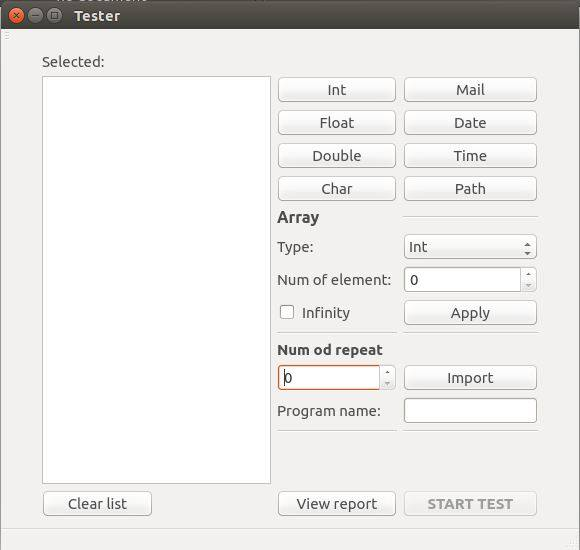
\includegraphics[scale=0.5]{korisnicki_interfejs.jpg}
\end{center}
\caption{Korisnički interfejs}
\label{fig:interfejs}
\end{figure}

Izveštaj rada se prikazuje u posebnoj formi u kojoj se pored informacija o vrednostima koje su korišćene za svaki test primer čuva i informacija o tome kako se program završio u obliku exit\_statusa. Čuvanje ovog izveštaja na lokalnom disku je omogućeno klikom na dugme sačuvaj.

\section{Zaključak}
\label{sec:zakljucak}
Predstavljene su vrste testiranja sa posebnim osvrtom na Fuzz tehniku. Opisani su koncepti crne, bele i sive strategije ispitivanja korektnosti softvera. Date su prednosti i nedostaci svakog od navedenih koncepata. Uočeno je da je Fuzz testiranje najpovoljniji pristup kada je potrebno proveriti ulazne podatke. Njegovom primenom se omogućava jednostavna i brza provera robusnosti paralelno sa razvojem koda. Navedena tehnika nije dovoljna za dokaz ispravnosti i potrebno je kombinovati je sa drugim vrstama jer je ona specijalizovana samo za kontrolu ulaznih podataka. \\

Drugi deo je posvećen našoj implementaciji Fuzz testera koji se koristi za programe napisane u jeziku C. Kao ulazne parametre testiranog programa je moguće zadati osnovne tipove podataka: int, double, float, char. Podržani su i neki od često korišćenih stringova: mail, vreme, datum, putanja. Data je i podrška za nizove čiji su elementi osnovni tipovi podataka. Posebna pažnja je posvećena pravljenju intuitivnog interfejsu radi što jednostavnije primene. Ostavljeno je prostora za dalja unapređenja, što može obuhvatiti detaljniju analizu već podržanih tipova podata, analizu novih tipova podataka u skladu sa potrebama i drugačiji način odabira test primera.
 
\addcontentsline{toc}{section}{Literatura}
\appendix
\bibliography{seminarski} 
\bibliographystyle{plain} 
\end{document}
